\documentclass[10pt]{beamer}

\usepackage{fontspec}
\setmainfont{Ubuntu}[]
\setsansfont{Ubuntu}[]
\setmonofont{Ubuntu Mono}[]

\usepackage{graphicx}
\graphicspath{ {../img/} }

\beamertemplatenavigationsymbolsempty

\title{Свойства BEAM}

\begin{document}

\begin{frame}
  \frametitle{Erlang Virtual Machine}
  Эликсир и Эрланг объединяет виртуальная машина EVM (Erlang~Virtual~Machine),
  \par \bigskip
  которую обычно называют \textbf{BEAM} (Bogdan's~Erlang~Abstract~Machine).
\end{frame}

\begin{frame}
  \frametitle{Erlang Virtual Machine}
  Операционная система в миниатюре:
  \begin{itemize}
  \item планировщик процессов,
  \item управление памятью,
  \item ввод-вывод,
  \item сетевой стек,
  \item и др.
  \end{itemize}
\end{frame}

\begin{frame}
  \frametitle{Erlang Virtual Machine}
  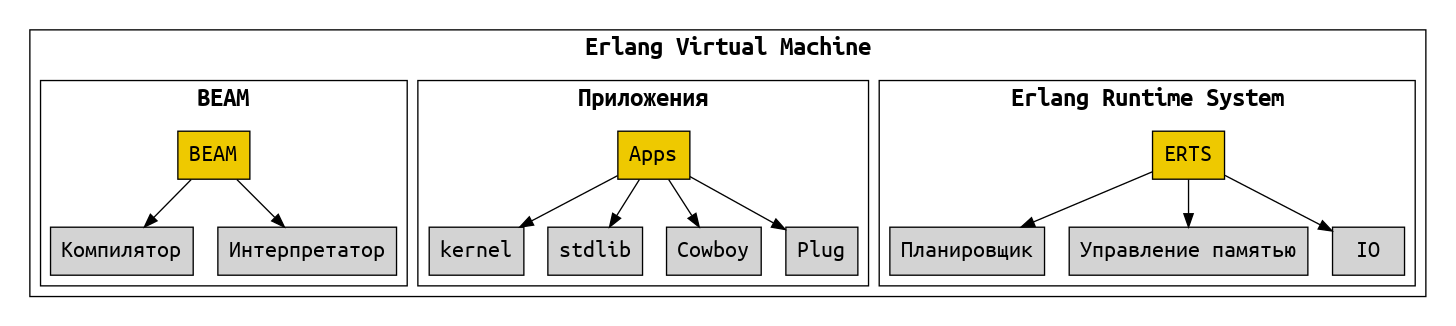
\includegraphics[scale=0.2]{evm}
\end{frame}

\begin{frame}
  \frametitle{Erlang Virtual Machine}
  Основные свойства машины:
  \begin{itemize}
  \item Многопоточность (Concurrency);
  \item Устойчивость к ошибкам (Fault Tolerance);
  \item Поддержка распределенных систем (Distribution);
  \item Горячее обновление кода (Hot Code Upgrade).
  \end{itemize}
\end{frame}

\begin{frame}
  \frametitle{Erlang Virtual Machine}
  Еще несколько свойств:
  \begin{itemize}
  \item Симметричная многопроцессорность (Symmetric~Multiprocessing);
  \item Модель акторов (Actor Model);
  \item Система реального времени (Soft Real Time);
  \item Сборщик мусора (Garbage Collector);
  \item Интерактивная консоль (Erlang/Elixir Shell);
  \item Трассировка (Tracing).
  \end{itemize}
\end{frame}

\begin{frame}
  \frametitle{Многопоточность}
  Процессы (thread) и планировщики (scheduler), независимые~от~ОС.
  \par \bigskip
  Процессы легковесные, их можно создавать десятки и~сотни~тысяч.
  \par \bigskip
\end{frame}
  
\begin{frame}
  \frametitle{Многопоточность}
  Каждый процесс имеет свою изолированную память, разделяемой памяти (shared memory) нет.
  \par \bigskip
  Процессы изолированы, блокировка или падение одного процесса не влияет на работу остальных.
  \par \bigskip
  Данные передаются отправкой сообщений (message passing).
\end{frame}

\begin{frame}
  \frametitle{Многопоточность}
  BEAM способна запускать до \textbf{134,217,727} ($2^{27}$) процессов.
  \par \bigskip
  Запуск нового процесса занимает \textbf{3-5 микросекунд}.
  \par \bigskip
  На старте процесс резервирует \textbf{2696 байт} памяти, включая стек, кучу~и~метаданные.
\end{frame}


\begin{frame}
  \frametitle{Многопоточность}
  Отдельный планировщик на каждом ядре CPU.
  \par \bigskip
  Балансируют нагрузку, передавая процессы друг другу.
\end{frame}

\begin{frame}
  \frametitle{Устойчивость к ошибкам}
  Исключения не основной способ обработки ошибок.
  \par \bigskip
  Основной способ -- это механизм мониторинга одних~процессов~другими.
  \par \bigskip
  \textbf{supervisor} (наблюдатель) и \textbf{worker} (рабочий процесс).
\end{frame}

\begin{frame}
  \frametitle{Устойчивость к ошибкам}
  Супервизоры наблюдают за рабочими процессами и~друг~за~другом.
  \par \bigskip
  Организованы в дерево, где узлами являются супервизоры, а~листьями~–~рабочие процессы.
\end{frame}

\begin{frame}
  \frametitle{Устойчивость к ошибкам}
  Следущий уровень устойчивости к ошибкам -- объединение узлов в кластер.
  \par \bigskip
  Если узел падает, то его функцию берет на себя другой узел.
\end{frame}


\begin{frame}
  \frametitle{Поддержка распределенных систем}
  Устойчивость к аппаратным авариям.
  \par \bigskip
  Железо выходит из строя не часто,
  \par \bigskip
  но в дата центре из сотен серверов это случается регулярно
  \par \bigskip
  и является штатной ситуацией.
\end{frame}

\begin{frame}
  \frametitle{Поддержка распределенных систем}
  Горизонтальное масштабирование позволяет
  \par \bigskip
  строить большие системы, справляющиеся
  \par \bigskip
  с большими нагрузками и большими данными.
\end{frame}

\begin{frame}
  \frametitle{Поддержка распределенных систем}
  Сетевая прозрачность (location transparency).
  \par \bigskip
  Процессы на одном узле и на разных узлах
  \par \bigskip
  общаются одинаково.
\end{frame}

\begin{frame}
  \frametitle{Поддержка распределенных систем}
  Доверенная среду (trusted environment).
  \par \bigskip
  Любой процесс может посылать любые сообщения кому угодно.
  \par \bigskip
  Любой код выполняется с равными правами, без ограничений.
\end{frame}

\begin{frame}
  \frametitle{Горячее обновление кода}
  Важно для телекомуникационного оборудования 80-90-х годов.
  \par \bigskip
  Обновление без прерывая обслуживания клиентов,
  \par \bigskip
  без разрыва текущих телефонных сессий.
\end{frame}

\begin{frame}
  \frametitle{Горячее обновление кода}
  В современном мире мы умеем поддерживать работу кластера
  \par \bigskip
  при выходе из стоя части узлов.
  \par \bigskip
  Используем это для обновления.
\end{frame}

\begin{frame}
  \frametitle{Горячее обновление кода}
  Полезно как инструмент разработки.
  \par \bigskip
  Используем локально на машине разработчика.
\end{frame}

\begin{frame}
  \frametitle{Симметричная многопроцессорность}
  BEAM эффективно использует все CPU.
  \par \bigskip
  Умеет перераспределять нагрузку между ними.
\end{frame}

\begin{frame}
  \frametitle{Симметричная многопроцессорность}
  Производительность линейно масштабируется с~ростом~числа~ядер.
  \par \bigskip
  Проверяли на чипах с 1024 ядрами.
  \par \bigskip
  Работает "из коробки".
\end{frame}

\begin{frame}
  \frametitle{Модель акторов}
  Один из способов реализации многопоточности.
\end{frame}

\begin{frame}
  \frametitle{Модель акторов}
  Система состоит из акторов,
  \par \bigskip
  которые действуют паралельно и независимо друг от друга,
  \par \bigskip
  имеют собственное состояние
  \par \bigskip
  и общаются друг с другом с помощью отправки сообщений.
\end{frame}

\begin{frame}
  \frametitle{Модель акторов}
  Для модель акторов реализована как библиотека.
  \par \bigskip
  Например, библиотека \textbf{Akka} для Java и Scala.
  \par \bigskip
  Но в BEAM эта модель поддерживается на уровне языка.
\end{frame}


\begin{frame}
  \frametitle{Система реального времени}
  Реагирует на запросы с гарантированным лимитом времени.
  \par \bigskip
  Нарушение лимита времени считается отказом~системы~(\textbf{hard~real-time}),
  \par \bigskip
  или снижением качества работы системы (\textbf{soft real-time}).
\end{frame}

\begin{frame}
  \frametitle{Система реального времени}
  Применяется в промышленности, транспорте, медицине.
  \par \bigskip
  Управление атомной электростанцией.
  \par \bigskip
  Авионика самолета.
  \par \bigskip
  Беспилотный автомобиль.
\end{frame}

\begin{frame}
  \frametitle{Система реального времени}
  BEAM поддерживает \textbf{soft real-time} благодаря:
  \begin{itemize}
  \item вытесняющей многозадачности (preemptive scheduling);
  \item изолированному IO;
  \item особенностям сборки мусора (garbage collection).
  \end{itemize}
\end{frame}

\begin{frame}
  \frametitle{Сборщик мусора}
  Отдельный для каждого процесса,
  \par \bigskip
  срабатывает независимо от других процессов,
  \par \bigskip
  в разные моменты времени.
  \par \bigskip
  Нет эффекта \textbf{stop world}.
\end{frame}

\begin{frame}
  \frametitle{Сборщик мусора}
  Вообще не запускается:
  \begin{itemize}
  \item короткоживущие процессы;
  \item долгоживущие процессы, потребляющие мало памяти.
  \end{itemize}
\end{frame}

\begin{frame}
  \frametitle{Сборщик мусора}
  Сборка мусора оказывает мало влияния
  \par \bigskip
  на производительность системы.
\end{frame}

\begin{frame}
  \frametitle{Интерактивная консоль}
  REPL-консоль (\textbf{R}ead, \textbf{E}val, \textbf{P}rint, \textbf{L}oop).
  \par \bigskip
  Работает не только локально, но и удаленно.
  \par \bigskip
  Интроспекция -- чтение информации о системе в~реальном~времени.
  \par \bigskip
  Можно взаимодействовать с production системой.
\end{frame}

\begin{frame}
  \frametitle{Трассировка}
  Получение событий системы в реальном времени:
  \begin{itemize}
  \item вызовы функций, аргументы, возвращаемые значения;
  \item работа планировщика;
  \item потреблении памяти;
  \item работа сборщиков мусора;
  \end{itemize}
\end{frame}

\begin{frame}
  \frametitle{Трассировка}
  Получение событий системы в реальном времени:
  \begin{itemize}
  \item жизненный цикл процессов (старт, остановка и др);
  \item отправка и получение сообщений;
  \item состояние памяти процессов.
  \end{itemize}
\end{frame}

\begin{frame}
  \frametitle{Трассировка}
  Теоретически можно узнать почти все о работе системы.
  \par \bigskip
  Cложность в том, чтобы найти именно ту информацию, которая~нужна.
\end{frame}

\end{document}
